\documentclass[11pt,a4paper]{article}
\usepackage[utf8]{inputenc}
\usepackage[czech]{babel}
\usepackage[T1]{fontenc}
\usepackage{amsmath}
\usepackage{amsfonts}
\usepackage{listings}
\usepackage{color}
\usepackage{epstopdf}
\usepackage{svg}
\definecolor{lightgray}{rgb}{.9,.9,.9}
\definecolor{darkgray}{rgb}{.4,.4,.4}
\definecolor{purple}{rgb}{0.65, 0.12, 0.82}
\usepackage{url}
\usepackage{amssymb}
\usepackage{graphicx}
\bibliographystyle{documentation}
\usepackage[left=2cm,right=2cm,top=2.5cm,bottom=2cm]{geometry}
\author{Stanislav Nechutný}
\begin{document}



\lstdefinelanguage{code}{
  keywords={},
  keywordstyle=\color{blue}\bfseries,
  ndkeywords={},
  ndkeywordstyle=\color{darkgray}\bfseries,
  identifierstyle=\color{black},
  sensitive=false,
  comment=[l]{//},
  morecomment=[s]{/*}{*/},
  commentstyle=\color{purple}\ttfamily,
  stringstyle=\color{red}\ttfamily,
  morestring=[b]',
  morestring=[b]"
}

\lstset{
   language=code,
   backgroundcolor=\color{lightgray},
   extendedchars=true,
   basicstyle=\footnotesize\ttfamily,
   showstringspaces=false,
   showspaces=false,
   numbers=left,
   numberstyle=\footnotesize,
   numbersep=9pt,
   tabsize=2,
   breaklines=true,
   showtabs=false,
   captionpos=b
}

\DeclareGraphicsExtensions{.pdf,.png,.jpg}

\newcommand{\slideRef}[1]{\textit{(IMS slide #1)}}
\newcommand{\code}[1]{\texttt{#1}}

	\begin{titlepage}

		\begin{center}

			\textsc{
				\Huge
					Vysoké učení technické v~Brně\\
				\huge
					Fakulta informačních technologií
			}\\

			\vspace{\stretch{0.320}}

			\LARGE
					IMS - Modelování a simulace\\
					3. Simulátor číslicových obvodů\\~\\
			\Huge{}
					Dokumentace
			\vspace{\stretch{0.650}}

		\end{center}

		{\Large
			30. listopadu 2015
			\hfill
			Stanislav Nechutný, Miloslav Smutka
		}

	\end{titlepage}

	\tableofcontents

	\pagebreak


	\section{Úvod a motivaci}
		Tato práce se zaměřuje na tvorbu simulátoru logických obvodů, který implementuje hradla \code{AND}, \code{OR}, \code{XOR}, \code{NOT}, \code{NOR}, \code{NAND}. Pro implementaci je zvolen jazyk C++ a jako vstup jednoduchý textový soubor, jehož formát je odvozen od netlistu. Blíže je vstupní formát popsán v této dokumentaci v kapitole \ref{netlist}.

		\subsection{Konzultace a zdroje}
			Chování logických členů v našem simulátoru modelů systému \slideRef{18} bylo konzultováno s panem Bc. Stanislavem Koskem, který je absolventem bakalářského studia na Fakultě elektronické a komunikačních technologií Vysokého učení technického v Brně a ve volném čase se zabývá návrhem logických obvodů a pokračuje v magisterském studiu. Jednalo se zejména o zjištění typických zpoždění hradel pro zajištění vhodné implementace simulátoru a dalších specifických vlastností hradel, které je třeba v simulaci zohlednit.

			Další informace o stavbě, chování a vlastnostech logickách hradel byla zjištěna ze stránek University of Surrey - Guildford, Eletricial and Electronix Engineering\cite{logicGate}. Dále pak byli použiti další internetové zdroje\cite{logicGateWiki}.

		\subsection{Ověřování validity modelu}
			Pro ověření validity modelu \slideRef{37} byla použita stavebnice Voltík III a Voltík II, které obsahují většinu, v tomto modelu implementovaných, logických hradel a je tedy možné sledovat průběh zapojení. Pro vizualizaci dat bylo využito připojení led diod a pro vizualizaci zpoždění zaznamenatelném lidským okem byli využity kondenzátory s různou kapacitou. Připojením výstupu logických hradel na osciloskop bylo sledováno odpovídající chování, jako u simulovaných a dochází tedy k ekvivalentnímu chování systémů \slideRef{26}. Podrobněji se validaci simulátoru zabýváme v kapitole \ref{validity} na straně \pageref{validity}.


	\section{Shrnutí relevantních faktů, zdroje informací}

		Logická hradla jsou elektronické součástky, které mají 1-n vstupů a jeden výstup. Vstupní a výstupní hodnotou je logická hodnota 1, nebo 0. Jejich chování je možno zapsat v booleově algebře. \cite{logicGate}

			\subsection{NOT}
				Negace. Jedná se o jednovstupový prvek, který má na výstupu opačnou hodnotu. V zápisu vstupního netlist sopuboru je zvolena identifikace \code{"NOT"}. Nastavené zpoždění na základě průzkumu je 10ns\cite{notSheet}.

			\subsection{AND}
				\label{and}
				Násobení. Prvek může mít 2-n vstupů. Výstupem je pak logická 1, jen v případě, že na všech vstupech je logická 1. V opačných případech je výstupem vždy logická 0. V zápisu vstupního netlist sopuboru je zvolena identifikace \code{"AND"}.  Nastavené zpoždění na základě průzkumu je 13ns\cite{andSheet}.

			\subsection{OR}
				\label{or}
				Sčítání. Prvek může mít 2-n vstupů. Výstupem je pak logická 1 pokuď alespoň jeden vstup nabývá hodnoty logická 1. V opačných případech je výstupem logická 0. V zápisu vstupního netlist sopuboru je zvolena identifikace \code{"OR"}.  Nastavené zpoždění na základě průzkumu je 11ns\cite{orSheet}.

			\subsection{XOR}
				Exkluzivita. Prvek má právě 2 vstupy. Výstupem je pak logická 1 pokuď na jednom vstupu je opačná hodnota druhého. V opačných případech je výstupem logická 0. V zápisu vstupního netlist sopuboru je zvolena identifikace \code{"XOR"}.  Nastavené zpoždění na základě průzkumu je 7ns\cite{xorSheet}.

			\subsection{NAND}
				Negovaný AND, který byl popsán v části \ref{and}. Takže výstup je vždy logická 1, kromě případů, kdy jsou všechny vstupy logická 1. V zápisu vstupního netlist sopuboru je zvolena identifikace \code{"NAND"}. Nastavené zpoždění na základě průzkumu je 20ns\cite{nandSheet}.

			\subsection{NOR}
				Negovaný OR, který byl popsán v části \ref{or}. Takže výstup je vždy logická 0, pokuď je alespoň jeden vstup logická 1. V zápisu vstupního netlist sopuboru je zvolena identifikace \code{"NOR"}.  Nastavené zpoždění na základě průzkumu je 13ns\cite{norSheet}.


		\subsection{Použité postupy}

			Použitým modelem signálů je dvouhodnotový \slideRef{277}, který je výrazně rychlý.

			Bylo zvoleno přiřaditelné zpoždění \slideRef{278} pro každý typ logického hradla. Tato varianta vychází ze zadání, ale je i zcela logickým požadavkem, které vychází z rozdílné vnitřní implementace hradel. Jsou uvnitř použité různé přechody v různém množství a tak samozřejmě dochází k odlišnostem ve zpoždění. Na tento fakt jsme byli také upozornění při konzultaci s Bc. Stanislavem Koskem.

			Krok byl zvolen 1 nanosekunda, aby nedošlo k problémům s detekcí změn stavových podmínek \slideRef{269}. Jak již víme například z předmětu Signály a systémy, tak vzorkovací frekvence by měla být alespoň dvojnásobná pro vhodné vzorkování na diskrétní hodnoty.

			Pro řešení zpětné vazby obvodů bylo zvoleno iterační řešení. Inicializace modelu \slideRef{279} vychází ze stavu, kdy v čase \code{T=0} je sepnut nejen vstup, ale i napájení logických členů, takže k nastavení jejich výstupů dochází v počáteční iteraci. Logické hradlo \code{NOT} tedy v čase \code{T=0} bude mít již na výstupu logickou 1, ale pokud má na vstup připojenu logickou 1, tak na výstupu se logická 0 objeví až v čase \code{T = zpoždění hradla}. Obdobné to bude u dalších negovaných hradel, jako například \code{NAND} apod.

			V případě hradel \code{AND}, \code{OR}, \code{XOR} pak bude výstup opačný, ale obdobný. Tedy v případě připojení dvou vstupů s logickou 1 v čase \code{T=0} bude výstupem logická 0 a tato hodnota se změní až po uplynutí zpoždění simulovaného hradla.

		\subsection{Původ postupů}
			Postupy byly získány z opory k předmětu Modelování a simulace \cite{imsSlide}, přednášek a democvičení. Následně jsme náš návrh konzultovali s 2 studenty magisterského oboru FIT VUT, kteří absolvovali předmět Modelování a simulace v akademickém roce 2014/2015 - Bc. Jiří Semmler a Bc. Jiří Kulda. Konkrétně se jednalo o zjištění, zda si nejsou vědomi skrytých překážek, které může námi zvolené řešení skrývat. Po vysvětlení našeho návrhu, bylo sděleno, že by se žádné komplikace při implementaci tohoto řešení neměly objevit.

			Na základě návrhu a informací v prezentaci \slideRef{276} byla zvolena implementace diskrétního modelu.


	\section{Koncepce metody, přístupu, modelu}

		Pro tvorbu byl zvolen simulátor uzavřeného systému \slideRef{30}, který nezohleďnuje vlivy prostředí. Bylo by velmi složité zadávat vliv prostředí (radiace, elektromagnetické záření apod.), které je naopak i v realném prostředí nežadoucí a eliminováno. Simulace je izomorfního systému \slideRef{27}, jelikož konkrétní prvky v simulaci odpovídají reálným prvkům.

		Model je koncipován deterministický \slideRef{32}, jelikož simuluje logické obvody, které mají deterministické chování a nejsou zde náhodné proměnné \slideRef{75}. Jak již bylo zmíněno v předchozím odstavci, tak se jedná o uzavřený systém, takže je zanedbáno rušení okolím.


	\section{Implementace metody, modelu}

		Pro implementaci byl zvolen kvaziparalelismus \slideRef{121} pro jeho jednoduchost a omezení počtu případných chyb vzniklých synchronizací paralelních procesů. Paralelismus by byl obtížně implementovatelný, jelikož chování jednoho členu systému závisí na předchozích výstupech ostatních.

		Na základě analýzy zadání a chování logických prvků bylo rozhodnuto, že bude využito konceptu objektově orientovaného programování \slideRef{168}, které nabízí jazyk C++. Každé simulované hradlo bude instancí třídy implementující konkrétní chování. Společné chování je implementováno v abstraktní třídě od které jednotlivá hradla dědí. Dalším typem objektu je vodič, který slouží k propojení vstupů a výstupů s hradly. Opět bude \textit{n} instancí v závislosti na vstupním souboru.

		Argumentem programu je množství požadovaného modelového času \slideRef{21}, který má být simulován. Jelikož je model implementován v prostředí číslicových systémů, tak je čas diskrétní \slideRef{22}. Program simulátoru je možné rozdělit do několika částí, které jsou zde rozebrány.

		\subsection{Načtení vstupního souboru}
			Vstupní soubor ve formátu netlistu (formát rozepsán v kapitole \ref{netlist}) je načítán po řádcích. Prvotně je sestaveno pole obsahující instance objektů reprezentující hradla. Jedná se o instance tříd \code{gateAnd}, \code{gateOr}, \code{gateNot} apod. Každá instance této třídy odpovíd jednomu hradlu ve vstupním souboru.

			Druhým krokem je vytvoření pole obsahující instance třídy \code{wire}, která slouží pro propojení vstupů a výstupů logických členů. Tato třída umožňuje připojit výstupy hradel, z kterých načítá výstupní hodnoty v čase \code{T}, a přenášet správnou hdonotu na vstupy.

			Třetím krokem načítání souboru je právě propojení instancí hradel s instancemi vodičů. V paměti tak vznikne orientovaný graf reprezentující strukturu simulovaného modelu. Během připojování je na vodič propagováno zpoždění hradel, které z vodiče načítají vstup, a uchovávána nejvyšší hodnota. Tato hodnota slouží pro alokaci kruhového bufferu hodnot, kterým je řešeno zpoždění prvků.

		\subsection{Simulace}
			Následná simulace nad vytvořenou strukturou probíhající ve smyčce je tvořena z dvou kroků. V prvním kroku probíhá vyhodnocení výstupu všech logických prvků. Hradlo v tomto kroku načte z vodičů připojených na vstup hodnotu, která na něm byla v čase \code{T - zpoždění}. Tato funkcionalita je implemntována ve třídě vodiče prostřednictvím kruhového bufferu o velikosti maximálního zpoždění vstupem připojených hradel. Na základě načtených hodnot a typu hradla je do atributu objektu nastaven výstup a propagován na výstup programu.

			V druhém kroku simulace jsou proiterovány všechny vodiče. Tento vodič načte výstupní hodnoty všech výstupem připojených hradel. Provede logický or a uloží výsledek do kruhového bufferu. Po provedení tohoto kroku se přechází k další iteraci cyklu simulace až po dosažení požadovaného simulačního času.

		\subsection{Netlist}
			\label{netlist}

			Simulovaný obvod je do programu nahrán ze souboru ve formátu netlistu\footnote{\url{https://en.wikipedia.org/wiki/Netlist}}. Netlist je ASCII soubor s příponou \code{.net}, který popisuje elektronické obvody, jejich součástky a propojení. Pro implementaci simulátoru jsme zvolili jednu z variant, jejichž specifikace je dostupná na adrese \url{http://www.expresspcb.com/ExpressPCBBin/NetlistFileFormat.pdf}.
			Skládá se ze čtyř bloků oddělených dvojitým odřádkováním (CRLF). Položky v blocích jsou odděleny jedním odřádkováním.

			První blok je hlavička. Ta má pevně daný formát a 8 řádků, na kterých se nachází následující položky

			\begin{enumerate}
				\item \code{"ExpressPCB Netlist"}
				\item Název software, který vytvořil netlist v uvozovkách (\code{"})
				\item Číslo udávající verzi formátu netlistu. V programu je využíván formát verze 1
				\item Počet varování, která byla zjištěna programem při tvorbě netlistu.
				\item Počet chyb, které byly zjištěny programem při tvorbě netlistu. Chybný netlist nelze simulovat, proto pokud byly nalezeny chyby, simulace neproběhne.
				\item Nevyužitý řádek, vždy by měl obsahovat pouze: \code{""}
				\item Nevyužitý řádek, vždy by měl obsahovat pouze: \code{""}
				\item Nevyužitý řádek, vždy by měl obsahovat pouze: \code{""}
			\end{enumerate}


			Druhým blokem je seznam využitých součástek. První řádek bloku musí být \code{"Part IDs Table"}. Na dalších řádcích jsou vypsané jednotlivé součástky. Každý řádek obsahuje tři položky v uvozovkách oddělené jedním či více bílými znaky. První položkou je název součástky, druhou typ a třetí položka je nevyužita a vždy by měla být prázdná. Typy součástek simulovatelných v aplikaci jsou následující: \code{AND}, \code{OR}, \code{NAND}, \code{NOR}, \code{NOT} a \code{INPUT}. \code{INPUT} je vstup, který je stále v logické 1.

\begin{lstlisting}[caption=Příklad bloku součástek]
"Part IDs Table"
"G1" "AND"  ""
"G2" "NAND" ""
"G3" "OR"   ""
\end{lstlisting}

			Třetím blokem je seznam kabelů. První řádek bloku musí být \code{"Net Names Table"}. Na dalších řádcích jsou vypsané kabely použité v zapojení. Každý řádek obsahuje dvě položky oddělené jedním či více bílými znaky. První položkou je název kabelu v uvozovkách. Druhou je pak číslo prvního řádku ve čtvrtém bloku netlistu, který jako první připojuje daný kabel.

\begin{lstlisting}[caption=Příklad bloku kabelů]
"Net Names Table"
"N01" 1
"N02" 3
"N03" 5
"N04" 7
\end{lstlisting}

			Čtvrtým blokem je seznam spojení kabelů a součástek. Na prvním řádku bloku musí být \code{"Net Connections Table"} a na dalších čtveřice číslic oddělená jedním či více bílými znaky. První číslice udává číslo řádku kabelu ve třetím bloku, který má být připojen. Druhá číslice udává číslo řádku součástky v druhém bloku, ke které má být připojen kabel. Třetí číslice udává číslo pinu součástky. Číslování pinů jsme si pro potřeby aplikace upravili následujícím způsobem. Nultý pin je vždy výstupem a je možné na něj napojit více kabelů. Ostatní piny jsou vstupy součástky číslované od jedné. Předpokládáme, že součástka má tolik vstupů, kolik je připojených pinů minus jeden, který je výstupem. Rozhodli jsme se tak proto, protože součástky mohou mít neurčitý počet vstupů, ale vždy pouze jeden výstup. Čtvrtá číslice obsahuje číslo řádku ve čtvrtém bloku, kde je připojován stejný kabel. Pokud již dále v zapojení není kabel použit, je na čtvrtém místě nula.

\begin{lstlisting}[caption=Příklad bloku propojení]
"Net Connections Table"
1 1 0 2
1 4 1 0
2 2 0 4
2 4 2 0
\end{lstlisting}


	\section{Experimentování}
		Po dokončení simulátoru jsme provedli několik experimentů pro ověření fungování simulátoru, při kterých jsme prováděli také sestavení obvodů a jejich sledování pomocí osciloskopu. V následujcí části jsou popsány některé vybrané testy.

		\subsection{Ověřování validity modelu}
			\label{validity}
			Pro ověření jsme navrhli několik následujících obvodů, které jsme také sestavili ve skutečnosti a ověřili, že je chování stejné. V prvním obvodu, který je znázorněn diagramem na obrázku \ref{fig:scheme1} jsme otestovali základní logické prvky a jejich fungování. Ověření simulace jsme provedli ručním vypracováním pravděpodobnostní tabulky a porovnali výstup se simulací. Graf průběhu je vidět na přiloženém obrázku \ref{fig:graf1}, kde je zobrazen průběh simulace pro prvních 50ns se zpožděními uvedenými dříve.


			\begin{figure}[!htb]
				\centering
					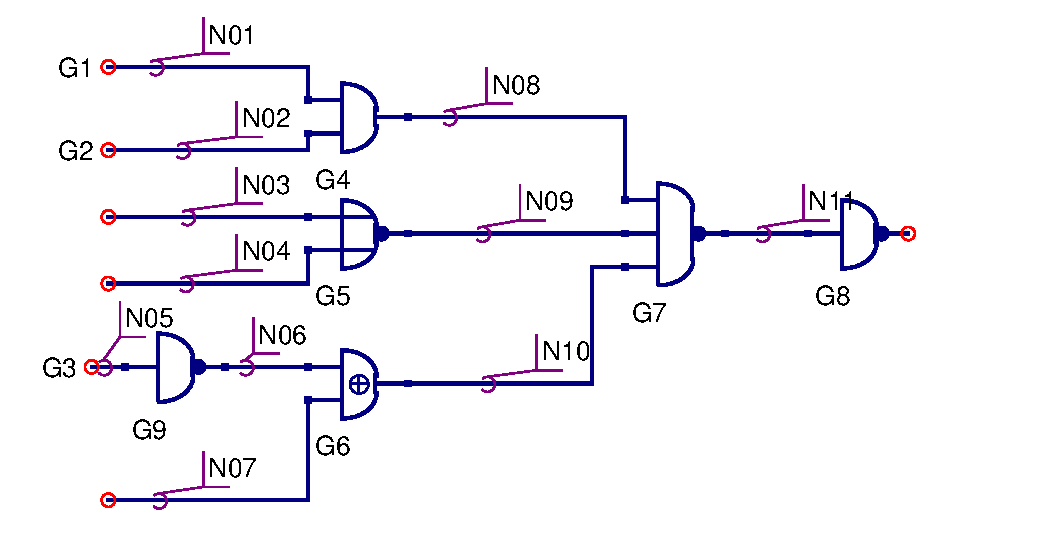
\includegraphics[scale=.5]{input1.eps}
					\caption{Schéma obvodu č. 1}
					\label{fig:scheme1}
			\end{figure}


			\begin{figure}[!htb]
				\centering
					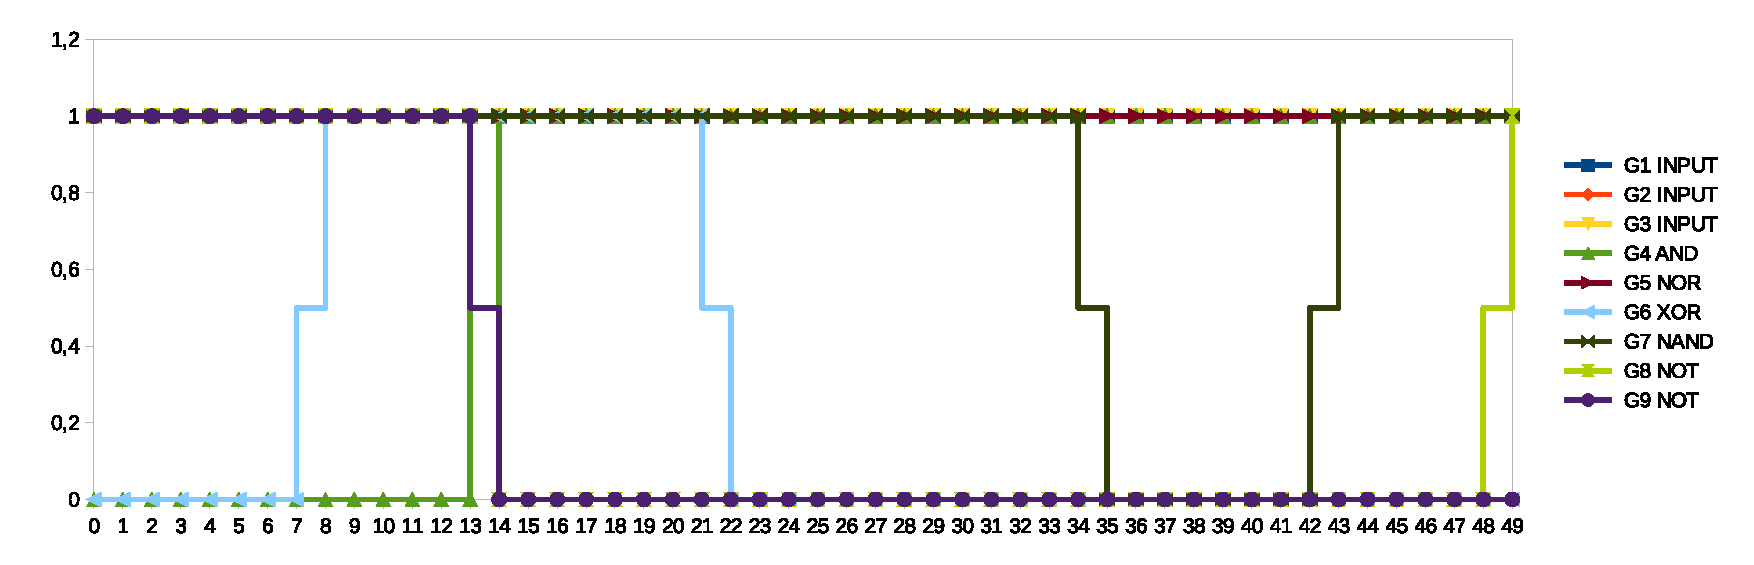
\includegraphics[scale=.6]{graf1.eps}
					\caption{Graf simulace obvodu č. 1}
					\label{fig:graf1}
			\end{figure}

			Dalším testovaným simulovaným obvodem bylo schéma na obrázku \ref{fig:scheme2}, ke kterému jsme opět připravili ručně pravdivostní tabulku. Dále jsme pak provedli zapojení tohoto obvodu a sledovali hodnoty pomocí osciloskopu. Graf simulace je přiložen jako obrázek \ref{fig:graf2} pro prvních 50ns.

			\begin{figure}[!htb]
					\centering
						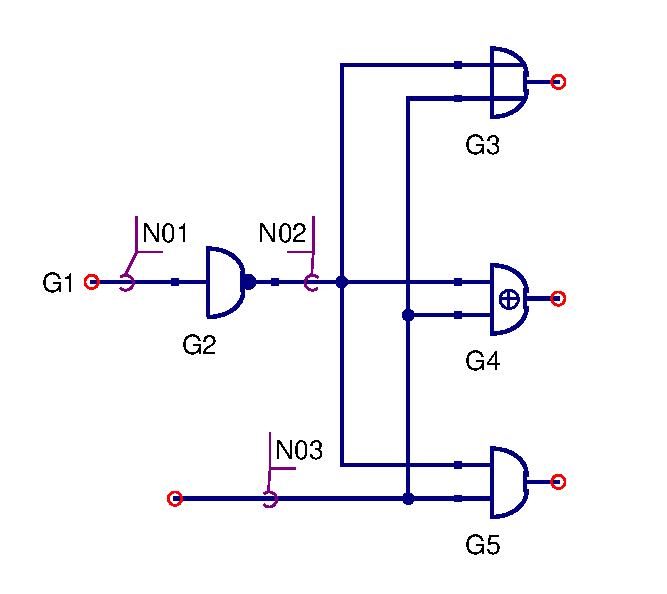
\includegraphics[scale=.5]{input2.eps}
						\caption{Schéma obvodu č. 2}
						\label{fig:scheme2}
			\end{figure}

			\begin{figure}[!htb]
				\centering
					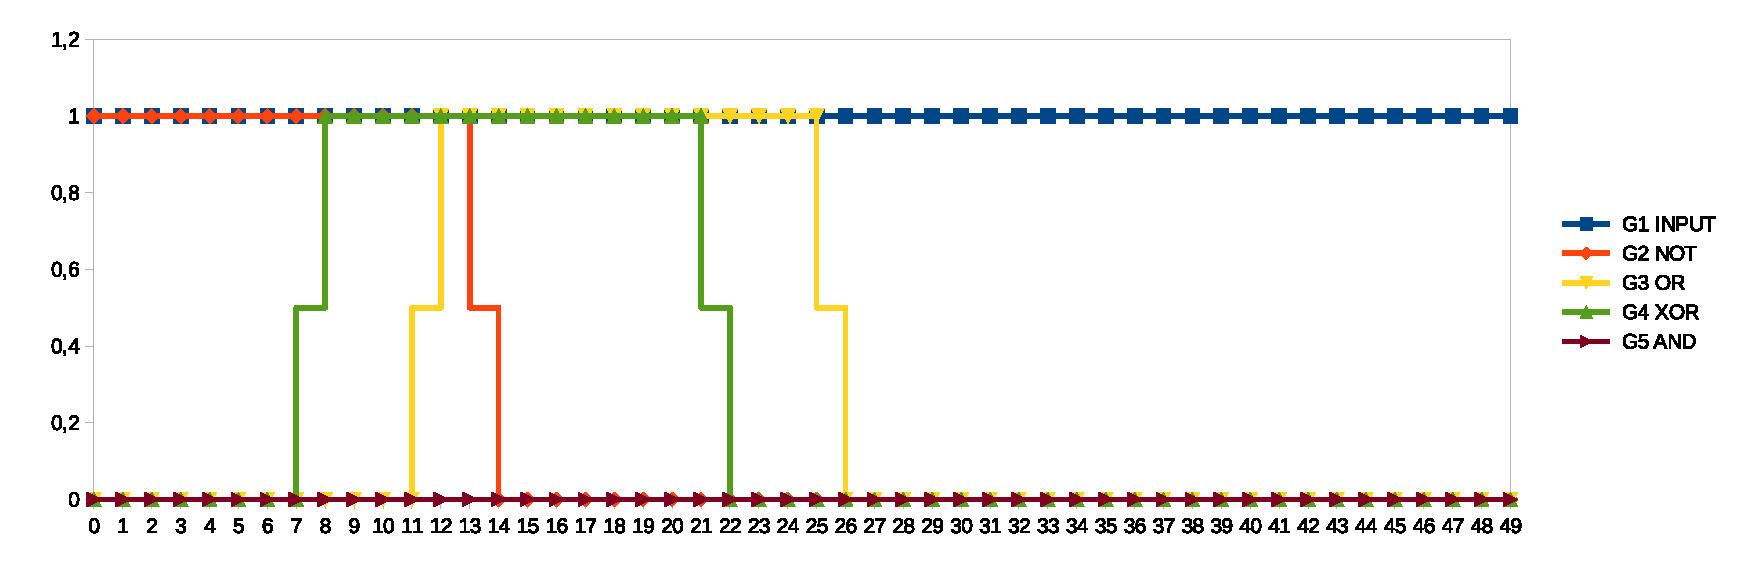
\includegraphics[scale=.6]{graf2.eps}
					\caption{Graf simulace obvodu č. 2}
					\label{fig:graf2}
			\end{figure}

			Po úspěšné simulaci základních obvodů jsme se rozhodli otestovat obvody se zpětnou vazbou. Testovaných schématem je obvod na obrázku \ref{fig:scheme3} s grafem výstupu na obrázku \ref{fig:graf3}, který se periodicky opakuje.

			\begin{figure}[!htb]
				\centering
					\includegraphics[scale=.5]{input3.eps}
					\caption{Schéma obvodu č. 3}
					\label{fig:scheme3}
			\end{figure}

			\begin{figure}[!htb]
				\centering
					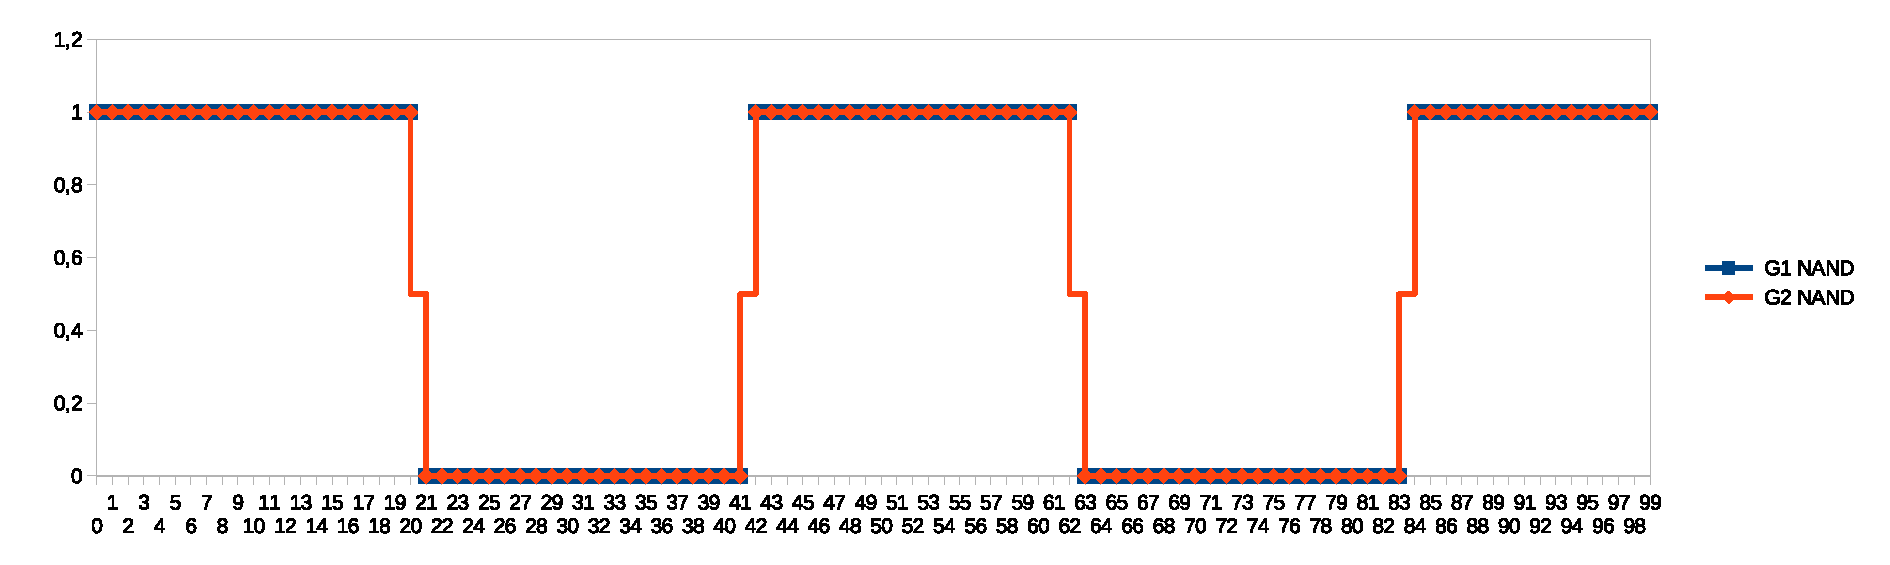
\includegraphics[scale=.55]{graf3.eps}
					\caption{Graf simulace obvodu č. 3}
					\label{fig:graf3}
			\end{figure}


	\section{Závěr}
		V rámci řešení této práce byl navrhnut a implementován simulátor logických obvodů. Bylo třeba se seznámit s fungováním logických členů a navrhnout simulátor tak, aby nejlépe odpovídal jejich skutečnému chování. Tomu předcházelo důkladné studium logických součástek na jejich elektronické i logické úrovni. Poté jsme postupně v sérii experimentů vyladili program tak, aby všechny jeho části co nejvíce odpovídaly realitě.

		Na závěr jsme provedli další testy, ve kterých jsme zkoumali, zda je naše simulace modelu validní a tento předpoklad se potvrdil.

	\section{Zdroje}
		\bibliography{documentation}


\end{document}
